\documentclass[8pt,ignorenonframetext,]{beamer}
\setbeamertemplate{caption}[numbered]
\setbeamertemplate{caption label separator}{: }
\setbeamercolor{caption name}{fg=normal text.fg}
\beamertemplatenavigationsymbolsempty
\usepackage{lmodern}
\usepackage{amssymb,amsmath}
\usepackage{ifxetex,ifluatex}
\usepackage{fixltx2e} % provides \textsubscript
\ifnum 0\ifxetex 1\fi\ifluatex 1\fi=0 % if pdftex
\usepackage[T1]{fontenc}
\usepackage[utf8]{inputenc}
\else % if luatex or xelatex
\ifxetex
\usepackage{mathspec}
\else
\usepackage{fontspec}
\fi
\defaultfontfeatures{Ligatures=TeX,Scale=MatchLowercase}
\fi
% use upquote if available, for straight quotes in verbatim environments
\IfFileExists{upquote.sty}{\usepackage{upquote}}{}
% use microtype if available
\IfFileExists{microtype.sty}{%
\usepackage{microtype}
\UseMicrotypeSet[protrusion]{basicmath} % disable protrusion for tt fonts
}{}
\newif\ifbibliography
\usepackage{color}
\usepackage{fancyvrb}
\newcommand{\VerbBar}{|}
\newcommand{\VERB}{\Verb[commandchars=\\\{\}]}
\DefineVerbatimEnvironment{Highlighting}{Verbatim}{commandchars=\\\{\}}
% Add ',fontsize=\small' for more characters per line
\usepackage{framed}
\definecolor{shadecolor}{RGB}{248,248,248}
\newenvironment{Shaded}{\begin{snugshade}}{\end{snugshade}}
\newcommand{\KeywordTok}[1]{\textcolor[rgb]{0.13,0.29,0.53}{\textbf{{#1}}}}
\newcommand{\DataTypeTok}[1]{\textcolor[rgb]{0.13,0.29,0.53}{{#1}}}
\newcommand{\DecValTok}[1]{\textcolor[rgb]{0.00,0.00,0.81}{{#1}}}
\newcommand{\BaseNTok}[1]{\textcolor[rgb]{0.00,0.00,0.81}{{#1}}}
\newcommand{\FloatTok}[1]{\textcolor[rgb]{0.00,0.00,0.81}{{#1}}}
\newcommand{\ConstantTok}[1]{\textcolor[rgb]{0.00,0.00,0.00}{{#1}}}
\newcommand{\CharTok}[1]{\textcolor[rgb]{0.31,0.60,0.02}{{#1}}}
\newcommand{\SpecialCharTok}[1]{\textcolor[rgb]{0.00,0.00,0.00}{{#1}}}
\newcommand{\StringTok}[1]{\textcolor[rgb]{0.31,0.60,0.02}{{#1}}}
\newcommand{\VerbatimStringTok}[1]{\textcolor[rgb]{0.31,0.60,0.02}{{#1}}}
\newcommand{\SpecialStringTok}[1]{\textcolor[rgb]{0.31,0.60,0.02}{{#1}}}
\newcommand{\ImportTok}[1]{{#1}}
\newcommand{\CommentTok}[1]{\textcolor[rgb]{0.56,0.35,0.01}{\textit{{#1}}}}
\newcommand{\DocumentationTok}[1]{\textcolor[rgb]{0.56,0.35,0.01}{\textbf{\textit{{#1}}}}}
\newcommand{\AnnotationTok}[1]{\textcolor[rgb]{0.56,0.35,0.01}{\textbf{\textit{{#1}}}}}
\newcommand{\CommentVarTok}[1]{\textcolor[rgb]{0.56,0.35,0.01}{\textbf{\textit{{#1}}}}}
\newcommand{\OtherTok}[1]{\textcolor[rgb]{0.56,0.35,0.01}{{#1}}}
\newcommand{\FunctionTok}[1]{\textcolor[rgb]{0.00,0.00,0.00}{{#1}}}
\newcommand{\VariableTok}[1]{\textcolor[rgb]{0.00,0.00,0.00}{{#1}}}
\newcommand{\ControlFlowTok}[1]{\textcolor[rgb]{0.13,0.29,0.53}{\textbf{{#1}}}}
\newcommand{\OperatorTok}[1]{\textcolor[rgb]{0.81,0.36,0.00}{\textbf{{#1}}}}
\newcommand{\BuiltInTok}[1]{{#1}}
\newcommand{\ExtensionTok}[1]{{#1}}
\newcommand{\PreprocessorTok}[1]{\textcolor[rgb]{0.56,0.35,0.01}{\textit{{#1}}}}
\newcommand{\AttributeTok}[1]{\textcolor[rgb]{0.77,0.63,0.00}{{#1}}}
\newcommand{\RegionMarkerTok}[1]{{#1}}
\newcommand{\InformationTok}[1]{\textcolor[rgb]{0.56,0.35,0.01}{\textbf{\textit{{#1}}}}}
\newcommand{\WarningTok}[1]{\textcolor[rgb]{0.56,0.35,0.01}{\textbf{\textit{{#1}}}}}
\newcommand{\AlertTok}[1]{\textcolor[rgb]{0.94,0.16,0.16}{{#1}}}
\newcommand{\ErrorTok}[1]{\textcolor[rgb]{0.64,0.00,0.00}{\textbf{{#1}}}}
\newcommand{\NormalTok}[1]{{#1}}
\usepackage{graphicx,grffile}
\makeatletter
\def\maxwidth{\ifdim\Gin@nat@width>\linewidth\linewidth\else\Gin@nat@width\fi}
\def\maxheight{\ifdim\Gin@nat@height>\textheight0.8\textheight\else\Gin@nat@height\fi}
\makeatother
% Scale images if necessary, so that they will not overflow the page
% margins by default, and it is still possible to overwrite the defaults
% using explicit options in \includegraphics[width, height, ...]{}
\setkeys{Gin}{width=\maxwidth,height=\maxheight,keepaspectratio}

% Prevent slide breaks in the middle of a paragraph:
\widowpenalties 1 10000
\raggedbottom

\AtBeginPart{
\let\insertpartnumber\relax
\let\partname\relax
\frame{\partpage}
}
\AtBeginSection{
\ifbibliography
\else
\let\insertsectionnumber\relax
\let\sectionname\relax
\frame{\sectionpage}
\fi
}
\AtBeginSubsection{
\let\insertsubsectionnumber\relax
\let\subsectionname\relax
\frame{\subsectionpage}
}

\setlength{\parindent}{0pt}
\setlength{\parskip}{6pt plus 2pt minus 1pt}
\setlength{\emergencystretch}{3em}  % prevent overfull lines
\providecommand{\tightlist}{%
\setlength{\itemsep}{0pt}\setlength{\parskip}{0pt}}
\setcounter{secnumdepth}{0}

\title{Happy R - Investigations Spatiales et Cartographiques}
\subtitle{Poursuite de la présentation de Jessica du 17/11/17}
\author{Eric \& Isabelle}
\date{23 mars 2018}

\begin{document}
\frame{\titlepage}

\section{Introduction}\label{introduction}

\begin{frame}[fragile]{Les données spatiales et R}

Les données spatiales se présentes sous la forme de:

\begin{itemize}
\item
  \texttt{vecteurs} (points, vecteurs, lignes, etc)
\item
  \texttt{raster} (pixels).
\end{itemize}

R permet de lire, d'écrire et de manipuler des données géoréférencées,
puis d'en faire l'analyse statistique. Nous avons repérés deux packages
de base :

\begin{itemize}
\item
  \texttt{sp} - classe de base pour gérér des données spatiales, en
  particulier vectorisées, mais aussi grilles.
\item
  \texttt{raster} - classes et outils pour manipuler des données sous
  forme raster.
\end{itemize}

\(+\) des outils, divers et variés, en particulier:

\begin{itemize}
\item
  \texttt{rgdal}: Interface R pour la library C/C++ de stat spatiales
  \texttt{gdal} (Geospatial Data Abstraction Library) pour lire et
  écrire des données spatialisées
\item
  \texttt{rgeos}: Interface R de la library \texttt{geos} (Geometry
  Engine Open Source) avec opérations de type ensemblistes
\end{itemize}

Bien d'autres packages spatiaux sur le CRAN!, voir -
\href{http://cran.r-project.org/web/views/Spatial.html}{Spatial task
view}

\end{frame}

\begin{frame}{Que fait-on aujourd'hui ?}

On étudie les packages \textbf{sp} puis \textbf{gstat}\ldots{}puis
\textbf{spacetime}

Il est possible de bricoler avec l'emploi des commandes uniquement de
base de R, telles que data.frame, image, etc\ldots{}.\textbf{MAIS}
pourquoi utiliser un package?

Accepter de perdre un peu de liberté indisciplinée ?

\begin{itemize}
\tightlist
\item
  pour travailler et partager avec d'autres collègues,
\item
  pour récupérer le travail d'autres collègues.
\item
  bénéficier des fondations et des extensions de \textbf{sp}
\end{itemize}

\begin{center}
  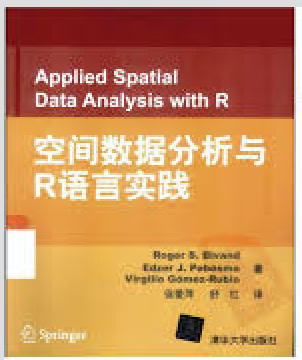
\includegraphics[width=0.3\textwidth]{figbookbivand.png}
\end{center}

Présentation inspirée des exemples de \href{http://asdar-book.org}{ce
bouquin} et du travail réalisé avec le réseau
\href{http://informatique-mia.inra.fr/resste/atelier}{RESSTE}

\end{frame}

\begin{frame}[fragile]{R n'est pas simplement la calculette du
statisticien}

\begin{Shaded}
\begin{Highlighting}[]
\NormalTok{cars$qspeed <-}\StringTok{ }\KeywordTok{cut}\NormalTok{(cars$speed, }\DataTypeTok{breaks=}\KeywordTok{quantile}\NormalTok{(cars$speed), }
                   \DataTypeTok{include.lowest=}\OtherTok{TRUE}\NormalTok{)}
\KeywordTok{par}\NormalTok{(}\DataTypeTok{mfrow=}\KeywordTok{c}\NormalTok{(}\DecValTok{1}\NormalTok{,}\DecValTok{2}\NormalTok{))}
\KeywordTok{plot}\NormalTok{(dist ~}\StringTok{ }\NormalTok{speed, }\DataTypeTok{data=}\NormalTok{cars)}
\KeywordTok{plot}\NormalTok{(dist ~}\StringTok{ }\NormalTok{qspeed, }\DataTypeTok{data=}\NormalTok{cars)}
\end{Highlighting}
\end{Shaded}

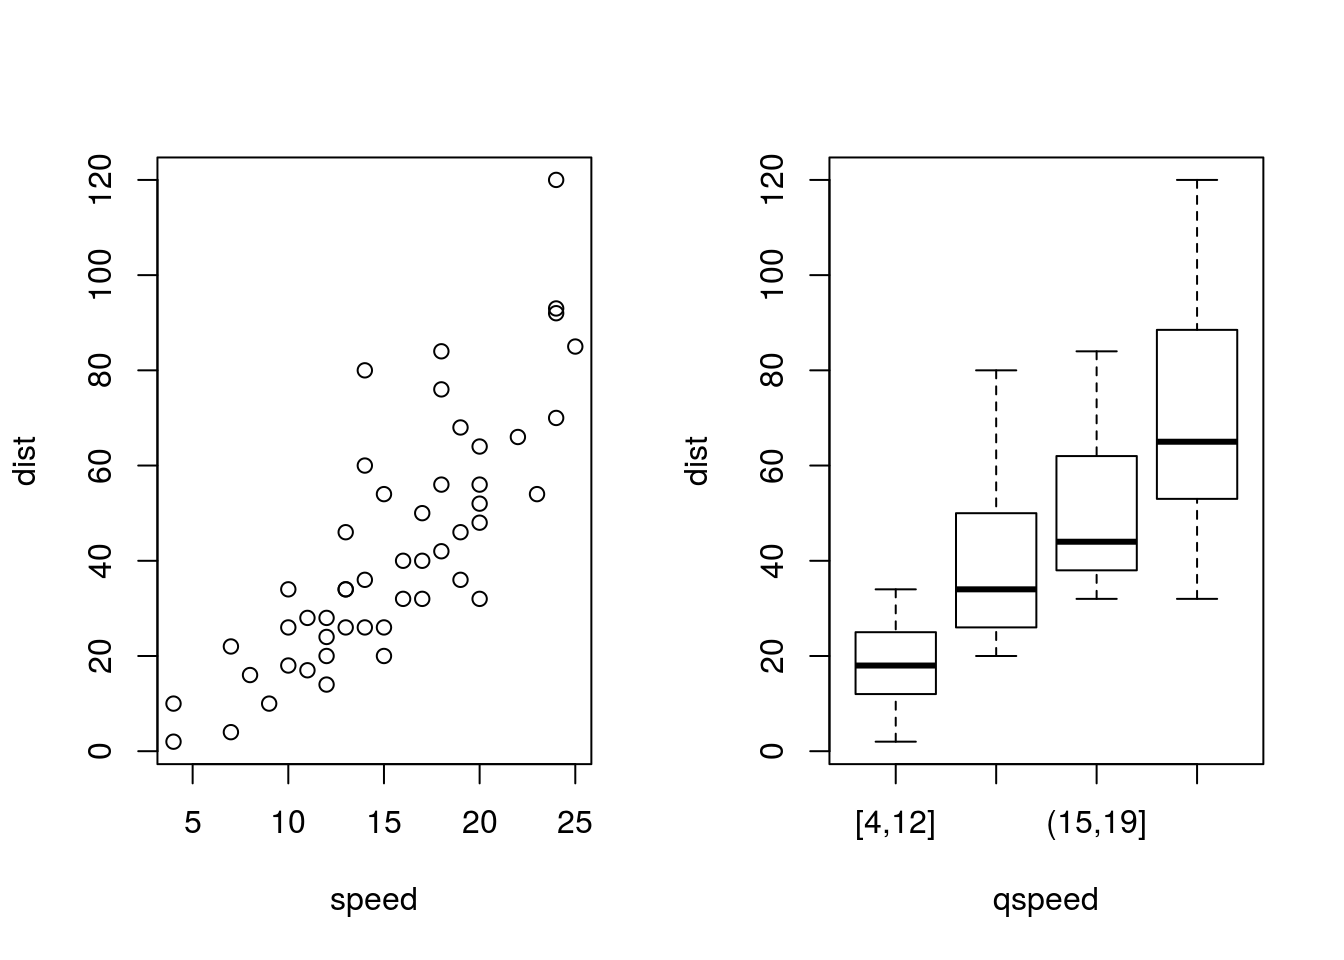
\includegraphics{happyR-230318_files/figure-beamer/calculette-1.pdf}

\begin{Shaded}
\begin{Highlighting}[]
\KeywordTok{par}\NormalTok{(}\DataTypeTok{mfrow=}\KeywordTok{c}\NormalTok{(}\DecValTok{1}\NormalTok{,}\DecValTok{1}\NormalTok{))}
\end{Highlighting}
\end{Shaded}

\end{frame}

\begin{frame}[fragile]{Le package sp définit des classes d'objet
explicitement spatialisés}

\begin{Shaded}
\begin{Highlighting}[]
\KeywordTok{library}\NormalTok{(sp)}
\KeywordTok{getClass}\NormalTok{(}\StringTok{"Spatial"}\NormalTok{)}
\NormalTok{## Class "Spatial" [package "sp"]}
\NormalTok{## }
\NormalTok{## Slots:}
\NormalTok{##                               }
\NormalTok{## Name:         bbox proj4string}
\NormalTok{## Class:      matrix         CRS}
\NormalTok{## }
\NormalTok{## Known Subclasses: }
\NormalTok{## Class "SpatialPoints", directly}
\NormalTok{## Class "SpatialMultiPoints", directly}
\NormalTok{## Class "SpatialGrid", directly}
\NormalTok{## Class "SpatialLines", directly}
\NormalTok{## Class "SpatialPolygons", directly}
\NormalTok{## Class "SpatialPointsDataFrame", by class "SpatialPoints", distance 2}
\NormalTok{## Class "SpatialPixels", by class "SpatialPoints", distance 2}
\NormalTok{## Class "SpatialMultiPointsDataFrame", by class "SpatialMultiPoints", distance 2}
\NormalTok{## Class "SpatialGridDataFrame", by class "SpatialGrid", distance 2}
\NormalTok{## Class "SpatialLinesDataFrame", by class "SpatialLines", distance 2}
\NormalTok{## Class "SpatialPixelsDataFrame", by class "SpatialPoints", distance 3}
\NormalTok{## Class "SpatialPolygonsDataFrame", by class "SpatialPolygons", distance 2}
\end{Highlighting}
\end{Shaded}

\end{frame}

\begin{frame}{Le package sp définit des classes d'objet explicitement
spatialisés}

\begin{itemize}
\tightlist
\item
  Points avec ou sans data : \emph{SpatialPoints} et
  \emph{SpatialPointsDataFrame}
\item
  Pixels avec ou sans data : \emph{SpatialPixels} et
  \emph{SpatialPixelsDataFrame}
\item
  Grilles avec ou sans data : \emph{SpatialGrid} et
  \emph{SpatialGridDataFrame}
\item
  Lignes avec ou sans data : \emph{SpatialGrid} et
  \emph{SpatialGridDataFrame}
\item
  Polygones : \emph{SpatialPolygons} et \emph{SpatialPolygonsDataFrame}
\end{itemize}

\end{frame}

\section{Spatial et SpatialPoints}\label{spatial-et-spatialpoints}

\begin{frame}[fragile]{La classe de base: Spatial}

Elle ne possède que 2 \emph{slots}

\begin{itemize}
\tightlist
\item
  un \emph{bounding box} en longitude/latitude
\item
  un objet de la classe \emph{CRS} (coordinate reference system), par
  défaut mise à CRS(as.character(NA)) . Voir plus tard ce qu'est un CRS.
\end{itemize}

\begin{Shaded}
\begin{Highlighting}[]
\KeywordTok{library}\NormalTok{(sp)}
\NormalTok{m <-}\StringTok{ }\KeywordTok{matrix}\NormalTok{(}\KeywordTok{c}\NormalTok{(-}\DecValTok{2}\NormalTok{,}\DecValTok{15}\NormalTok{,}\DecValTok{10}\NormalTok{,}\DecValTok{40}\NormalTok{), }\DataTypeTok{ncol=}\DecValTok{2}\NormalTok{, }\DataTypeTok{dimnames=}\KeywordTok{list}\NormalTok{(}\OtherTok{NULL}\NormalTok{, }\KeywordTok{c}\NormalTok{(}\StringTok{"min"}\NormalTok{, }\StringTok{"max"}\NormalTok{)))}
\NormalTok{crs <-}\StringTok{ }\KeywordTok{CRS}\NormalTok{(}\DataTypeTok{projargs=}\KeywordTok{as.character}\NormalTok{(}\OtherTok{NA}\NormalTok{))}
\NormalTok{crs}
\NormalTok{## CRS arguments: NA}
\NormalTok{S <-}\StringTok{ }\KeywordTok{Spatial}\NormalTok{(}\DataTypeTok{bbox=}\NormalTok{m, }\DataTypeTok{proj4string=}\NormalTok{crs)}
\NormalTok{S}
\NormalTok{## An object of class "Spatial"}
\NormalTok{## Slot "bbox":}
\NormalTok{##      min max}
\NormalTok{## [1,]  -2  10}
\NormalTok{## [2,]  15  40}
\NormalTok{## }
\NormalTok{## Slot "proj4string":}
\NormalTok{## CRS arguments: NA}
\end{Highlighting}
\end{Shaded}

\end{frame}

\begin{frame}[fragile]{Pour la suite de l'exposé, on s'appuie sur le
jeux de données MEUSE}

\begin{Shaded}
\begin{Highlighting}[]
\CommentTok{# check for example data}
\KeywordTok{data}\NormalTok{(meuse) }\CommentTok{# mesures de métaux lourds dans la meuse}
\KeywordTok{str}\NormalTok{(meuse) }\CommentTok{# 155 observations et 14 variables}
\NormalTok{## 'data.frame':    155 obs. of  14 variables:}
\NormalTok{##  $ x      : num  181072 181025 181165 181298 181307 ...}
\NormalTok{##  $ y      : num  333611 333558 333537 333484 333330 ...}
\NormalTok{##  $ cadmium: num  11.7 8.6 6.5 2.6 2.8 3 3.2 2.8 2.4 1.6 ...}
\NormalTok{##  $ copper : num  85 81 68 81 48 61 31 29 37 24 ...}
\NormalTok{##  $ lead   : num  299 277 199 116 117 137 132 150 133 80 ...}
\NormalTok{##  $ zinc   : num  1022 1141 640 257 269 ...}
\NormalTok{##  $ elev   : num  7.91 6.98 7.8 7.66 7.48 ...}
\NormalTok{##  $ dist   : num  0.00136 0.01222 0.10303 0.19009 0.27709 ...}
\NormalTok{##  $ om     : num  13.6 14 13 8 8.7 7.8 9.2 9.5 10.6 6.3 ...}
\NormalTok{##  $ ffreq  : Factor w/ 3 levels "1","2","3": 1 1 1 1 1 1 1 1 1 1 ...}
\NormalTok{##  $ soil   : Factor w/ 3 levels "1","2","3": 1 1 1 2 2 2 2 1 1 2 ...}
\NormalTok{##  $ lime   : Factor w/ 2 levels "0","1": 2 2 2 1 1 1 1 1 1 1 ...}
\NormalTok{##  $ landuse: Factor w/ 15 levels "Aa","Ab","Ag",..: 4 4 4 11 4 11 4 2 2 15 ...}
\NormalTok{##  $ dist.m : num  50 30 150 270 380 470 240 120 240 420 ...}
\end{Highlighting}
\end{Shaded}

\end{frame}

\begin{frame}[fragile]{Spatial points}

On utilise les 2 colonnes du data.frame meuse renseignant les
coordonnées géographiques pour en faire un objet \emph{SpatialPoints}

\begin{Shaded}
\begin{Highlighting}[]
\CommentTok{# check for example data}
\NormalTok{coords <-}\StringTok{ }\KeywordTok{SpatialPoints}\NormalTok{(meuse[, }\KeywordTok{c}\NormalTok{(}\StringTok{"x"}\NormalTok{, }\StringTok{"y"}\NormalTok{)]) }
\KeywordTok{summary}\NormalTok{(coords)}
\NormalTok{## Object of class SpatialPoints}
\NormalTok{## Coordinates:}
\NormalTok{##      min    max}
\NormalTok{## x 178605 181390}
\NormalTok{## y 329714 333611}
\NormalTok{## Is projected: NA }
\NormalTok{## proj4string : [NA]}
\NormalTok{## Number of points: 155}
\end{Highlighting}
\end{Shaded}

\end{frame}

\begin{frame}{Exercice à vous de jouer}

\begin{block}{Merci à Maxime Beauchamp et Laure Malherbe de l'Ineris}

\begin{center}
  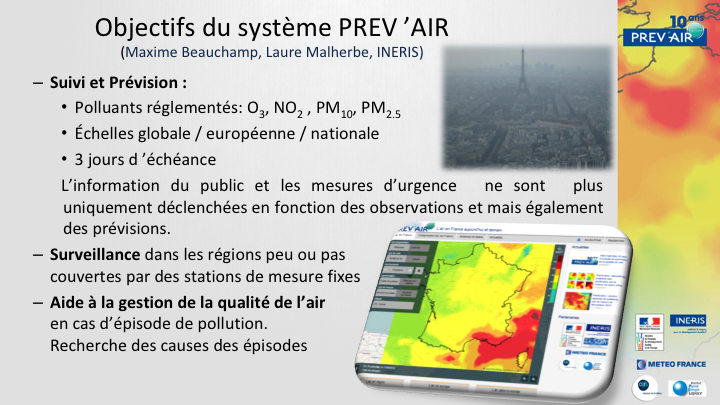
\includegraphics[width=1\textwidth]{figINERIS1.png}
\end{center}

\end{block}

\end{frame}

\begin{frame}{Exercice à vous de jouer}

\begin{center}
  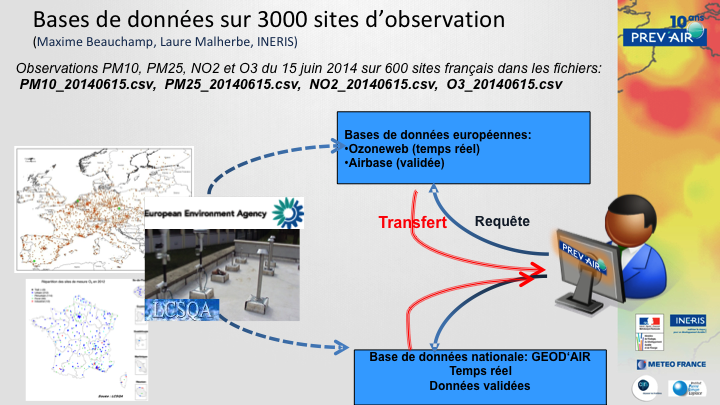
\includegraphics[width=1\textwidth]{figINERIS3.png}
\end{center}

\end{frame}

\begin{frame}{Exercice à vous de jouer}

\begin{center}
  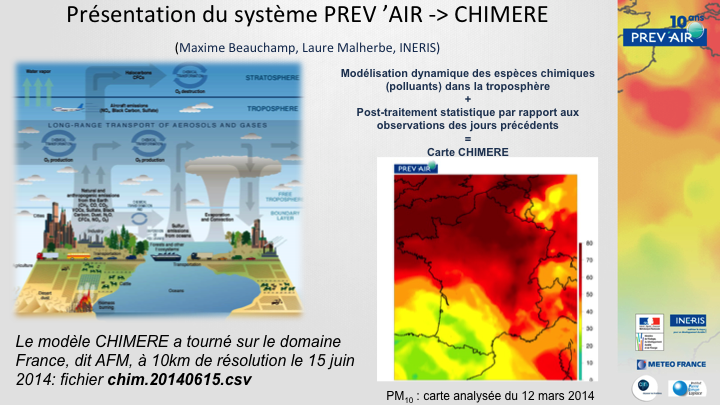
\includegraphics[width=1\textwidth]{figINERIS2.png}
\end{center}

\end{frame}

\begin{frame}[fragile]{Exercice 1}

Lire les stations de suivi de la pollution atmosphérique en PM10, PM25 ,
NO2 et O3 dans le fichier \textbf{AirBase\_v7\_stations.csv}.

Extraire leur coordonnées, jeter les doublons et sélectionner les
stations de France métropolitaine. En faire un objet
\emph{SpatialPoints} et les représenter. On pourra extraire un fond de
carte de la France par les commandes R suivantes:

\begin{Shaded}
\begin{Highlighting}[]
\KeywordTok{library}\NormalTok{(cshapes)}
\NormalTok{## Loading required package: maptools}
\NormalTok{## Checking rgeos availability: TRUE}
\NormalTok{## Loading required package: plyr}
\NormalTok{cs<-}\KeywordTok{cshp}\NormalTok{()}
\KeywordTok{row.names}\NormalTok{(cs)=}\KeywordTok{paste}\NormalTok{(}\KeywordTok{as.character}\NormalTok{(cs$CNTRY_NAME),}\DecValTok{1}\NormalTok{:}\DecValTok{244}\NormalTok{)}
\NormalTok{numfrance=}\KeywordTok{grep}\NormalTok{(}\StringTok{'France'}\NormalTok{,}\KeywordTok{row.names}\NormalTok{(cs)) }\CommentTok{#=106}
\NormalTok{cowcodefrance=cs$COWCODE[}\DecValTok{106}\NormalTok{]}
\NormalTok{france <-}\StringTok{ }\NormalTok{cs[cs$COWCODE==cowcodefrance,]}
\end{Highlighting}
\end{Shaded}

\end{frame}

\begin{frame}[fragile]{Spatial points data frame}

Retour à Meuse. On ajoute aux coordonnées géographiques les données pour
en faire un objet \emph{SpatialPointsDataFrame}. Ca se comporte comme un
dataframe!

\begin{Shaded}
\begin{Highlighting}[]
\NormalTok{meuse_sp <-}\StringTok{ }\KeywordTok{SpatialPointsDataFrame}\NormalTok{(coords, meuse)}
\KeywordTok{names}\NormalTok{(meuse_sp)}
\NormalTok{##  [1] "x"       "y"       "cadmium" "copper"  "lead"    "zinc"   }
\NormalTok{##  [7] "elev"    "dist"    "om"      "ffreq"   "soil"    "lime"   }
\NormalTok{## [13] "landuse" "dist.m"}
\KeywordTok{is}\NormalTok{(meuse_sp)}
\NormalTok{## [1] "SpatialPointsDataFrame" "SpatialPoints"         }
\NormalTok{## [3] "Spatial"}
\KeywordTok{is}\NormalTok{(meuse)}
\NormalTok{## [1] "data.frame" "list"       "oldClass"   "vector"}
\CommentTok{#str(meuse_sp)}
\end{Highlighting}
\end{Shaded}

On aurait pu faire plus direct:

\begin{Shaded}
\begin{Highlighting}[]
\NormalTok{meuse_sp2 <-}\StringTok{ }\NormalTok{meuse}
\KeywordTok{coordinates}\NormalTok{(meuse_sp2) <-}\StringTok{ }\ErrorTok{~}\NormalTok{x+y }
\CommentTok{# str(meuse_sp2)}
\KeywordTok{is}\NormalTok{(meuse_sp2)}
\NormalTok{## [1] "SpatialPointsDataFrame" "SpatialPoints"         }
\NormalTok{## [3] "Spatial"}
\end{Highlighting}
\end{Shaded}

\end{frame}

\begin{frame}{Exercice 2}

Lire les données de pollution atmosphérique du 15 juin 2014 en PM10,
PM25 , NO2 et O3 pour les stations actives de France métropolitaine dans
les fichiers \textbf{PM10\_20140615.csv}, \textbf{PM25\_20140615.csv},
\textbf{NO2\_20140615.csv} et \textbf{03\_20140615.csv} . Les données
manquantes sont codées -999.

On pourra utiliser les packages \emph{tidyR} et \emph{data.table} pour
avoir recours à la méthode \emph{merge}. Créer un objet
\emph{SpatialPointsDataFrame} contenant les enregistrements géolocalisés
de PM10, PM25 , NO2 et O3 pour les stations actives au 15 juin 2014 dont
on conservera le type et l'aire.

\end{frame}

\begin{frame}{Recap: ASDAR page 35}

\begin{center}
  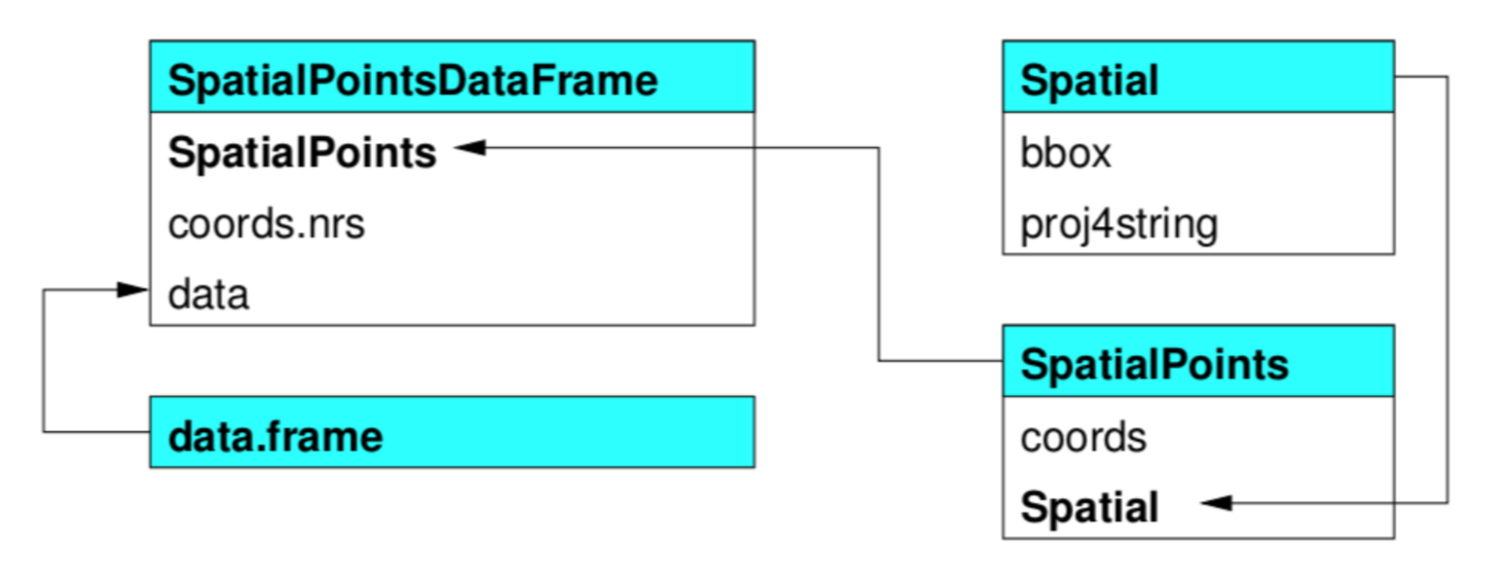
\includegraphics[width=1\textwidth]{figSpatialPoints.png}
\end{center}

\end{frame}

\section{SpatialGrids \&
SpatialPixels}\label{spatialgrids-spatialpixels}

\begin{frame}[fragile]{Spatial grids \& pixels}

2 representations pour les data sur une grille régulière rectangualire,
orientée N-S et E-W: \emph{SpatialPixels} et \emph{SpatialGrid}

\begin{itemize}
\item
  SpatialPixels comme SpatialPoints, mais avec coordonnées equi-espacées
\item
  SpatialPixelsDataFrame = SpatialPixels+data
\item
  SpatialGridDataFrame = grille entiere et NA où manquantes
\end{itemize}

\begin{Shaded}
\begin{Highlighting}[]
 \KeywordTok{data}\NormalTok{(meuse.grid)}
 \NormalTok{coords <-}\StringTok{ }\KeywordTok{SpatialPixels}\NormalTok{(}\KeywordTok{SpatialPoints}\NormalTok{(meuse.grid[, }\KeywordTok{c}\NormalTok{(}\StringTok{"x"}\NormalTok{,}\StringTok{"y"}\NormalTok{)]))}
\NormalTok{meuse_spx <-}\StringTok{ }\KeywordTok{SpatialPixelsDataFrame}\NormalTok{(coords, meuse.grid)}
\KeywordTok{names}\NormalTok{(meuse_spx)}
\NormalTok{## [1] "x"      "y"      "part.a" "part.b" "dist"   "soil"   "ffreq"}
\KeywordTok{slot}\NormalTok{(meuse_spx, }\StringTok{"grid"}\NormalTok{)}
\NormalTok{##                        x      y}
\NormalTok{## cellcentre.offset 178460 329620}
\NormalTok{## cellsize              40     40}
\NormalTok{## cells.dim             78    104}
\KeywordTok{object.size}\NormalTok{(meuse_spx) }
\NormalTok{## 565952 bytes}
\KeywordTok{dim}\NormalTok{(}\KeywordTok{slot}\NormalTok{(meuse_spx, }\StringTok{"data"}\NormalTok{))}
\NormalTok{## [1] 3103    7}
\end{Highlighting}
\end{Shaded}

\end{frame}

\begin{frame}[fragile]{Spatial grids}

On peut convertir un \emph{SpatialPixels} en un \emph{SpatialGrid}, ce
qui économise de la place de stockage:

\begin{Shaded}
\begin{Highlighting}[]
\NormalTok{meuse_sg <-}\StringTok{ }\NormalTok{meuse_spx}
\KeywordTok{fullgrid}\NormalTok{(meuse_sg) <-}\StringTok{ }\OtherTok{TRUE} 
\KeywordTok{slot}\NormalTok{(meuse_sg, }\StringTok{"grid"}\NormalTok{)}
\NormalTok{##                        x      y}
\NormalTok{## cellcentre.offset 178460 329620}
\NormalTok{## cellsize              40     40}
\NormalTok{## cells.dim             78    104}
\KeywordTok{class}\NormalTok{(}\KeywordTok{slot}\NormalTok{(meuse_sg, }\StringTok{"grid"}\NormalTok{))}
\NormalTok{## [1] "GridTopology"}
\NormalTok{## attr(,"package")}
\NormalTok{## [1] "sp"}
\KeywordTok{object.size}\NormalTok{(meuse_sg)}
\NormalTok{## 395808 bytes}
\KeywordTok{dim}\NormalTok{(}\KeywordTok{slot}\NormalTok{(meuse_sg, }\StringTok{"data"}\NormalTok{))}
\NormalTok{## [1] 8112    7}
\KeywordTok{par}\NormalTok{(}\DataTypeTok{mfrow=}\KeywordTok{c}\NormalTok{(}\DecValTok{1}\NormalTok{,}\DecValTok{1}\NormalTok{))}
\end{Highlighting}
\end{Shaded}

\end{frame}

\begin{frame}[fragile]{Spatial grids}

Interpolons par ``inverse distance weighting'' un objet
\emph{SpatialPointsDataFrame}

\begin{Shaded}
\begin{Highlighting}[]
\KeywordTok{library}\NormalTok{(gstat)}
\NormalTok{meuse_sg$zincIDW <-}\StringTok{ }\KeywordTok{idw}\NormalTok{(zinc~}\DecValTok{1}\NormalTok{,meuse_sp, meuse_sg)$var1.pred }
\NormalTok{## [inverse distance weighted interpolation]}
\CommentTok{#interpolation par un poids inverse à la distance}
    \KeywordTok{bubble}\NormalTok{(meuse_sp, }\StringTok{"zinc"}\NormalTok{,}\DataTypeTok{col =} \KeywordTok{c}\NormalTok{(}\StringTok{"white"}\NormalTok{, }\StringTok{"orange"}\NormalTok{))}
\end{Highlighting}
\end{Shaded}

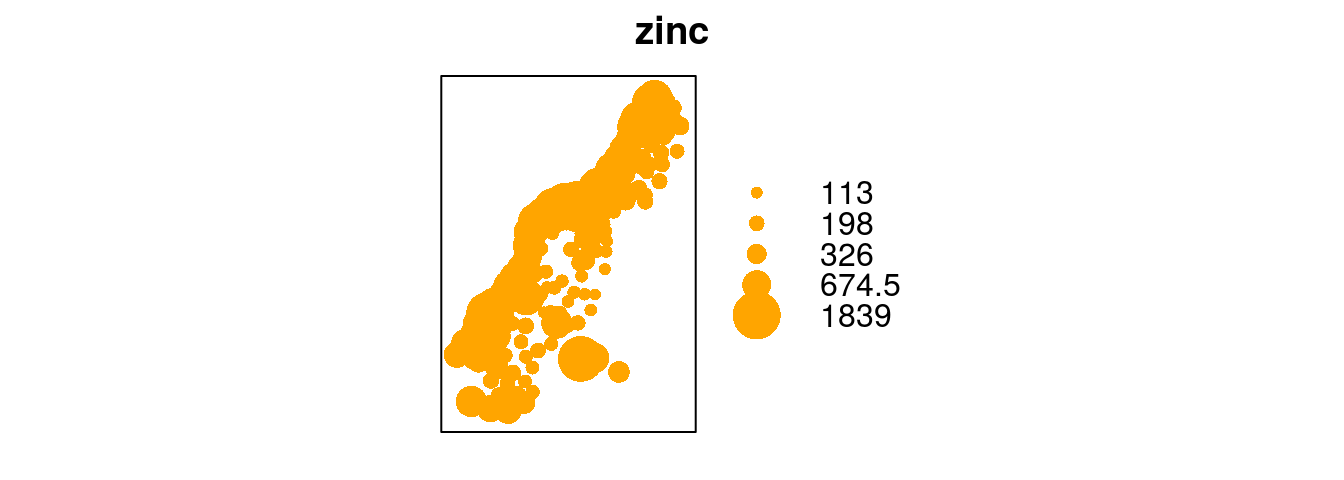
\includegraphics{happyR-230318_files/figure-beamer/faireSpatialPixelsDataFrame3-1.pdf}

\end{frame}

\begin{frame}[fragile]{Spatial grids}

L'interpolation par ``inverse distance weighting'' d'un objet
\emph{SpatialPointsDataFrame} crée un objet \emph{SpatialGridDataFrame}:

\begin{Shaded}
\begin{Highlighting}[]
    \KeywordTok{image}\NormalTok{(meuse_sg,}\StringTok{"zincIDW"}\NormalTok{, }\DataTypeTok{col=} \KeywordTok{terrain.colors}\NormalTok{(}\DecValTok{7}\NormalTok{))}
\end{Highlighting}
\end{Shaded}

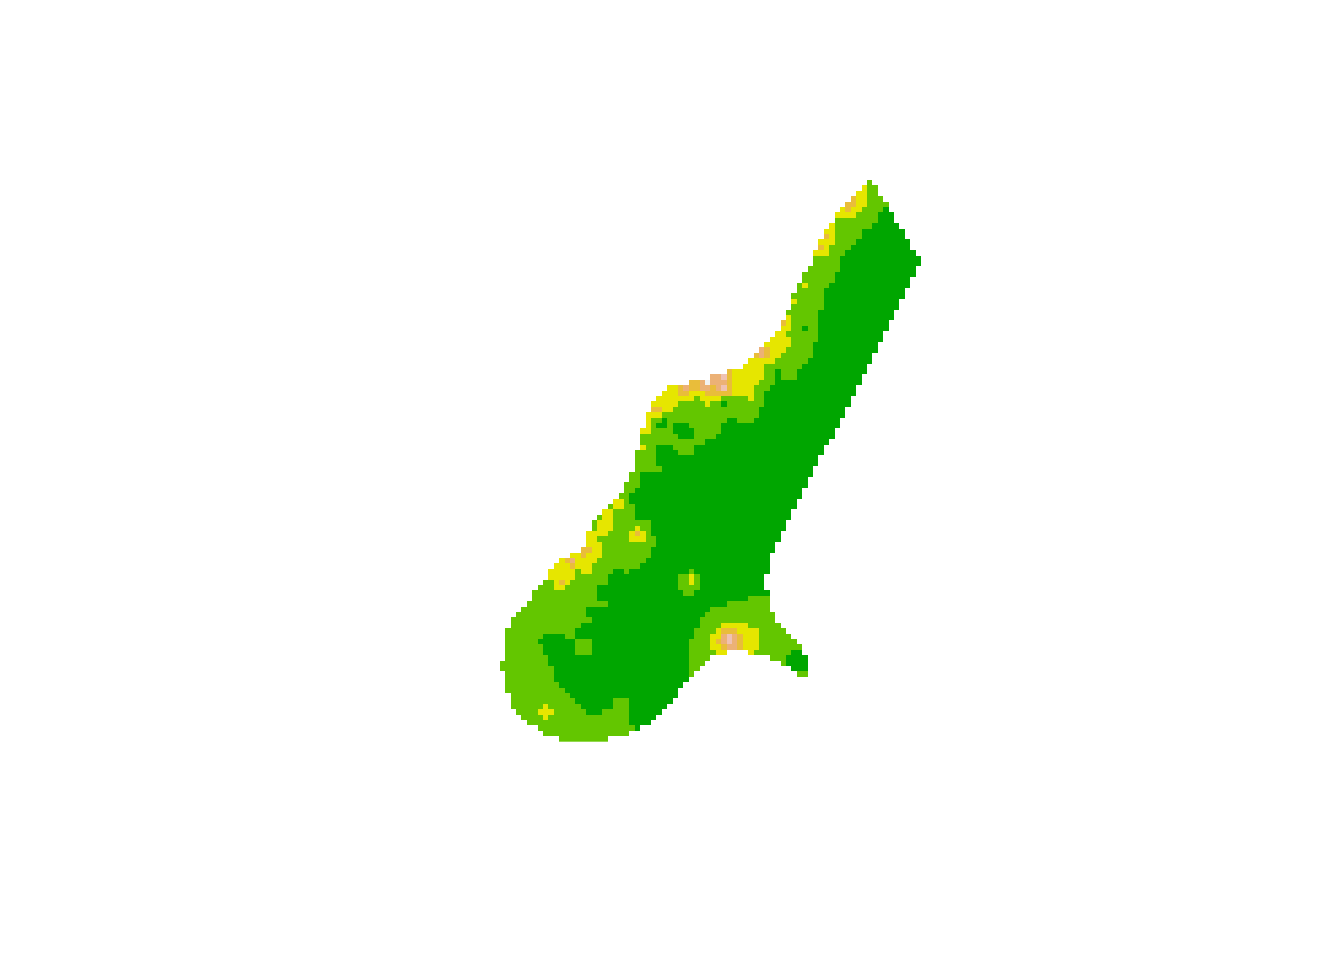
\includegraphics{happyR-230318_files/figure-beamer/faireSpatialPixelsDataFrame4-1.pdf}

\end{frame}

\begin{frame}{Exercice 3}

\begin{itemize}
\item
  Lire le champ de pollution atmosphérique du 15 juin 2014 en PM10, PM25
  , NO2 et O3 prévues par le code numérique CHIMERE sur une grille
  régulière recouvrant la France métropolitaine dans le fichier
  \textbf{chim.20140615.csv}. Vérifier que l'écartement entre les points
  est régulier et le corriger si nécessaire. Faire une représentation
  graphique du champ de prévisions de PM25 du 15 juin 2014 sur laquelle
  on pourra tracer le fond de carte des contours de la France
  métropolitaine. Créer un objet \emph{SpatialPixelDataFrame} . Quelle
  est sa taille? Le transformer en un objet \emph{SpatialGridDataFrame}.
  A-t-on économisé de l'espace de stockage?
\item
  Interpoler par ``inverse distance weighting'' (en supposant qu'un
  écart d'un degré de latitude correspond à celui d'un degré de
  longiture) les observations de PM25 (un objet
  \emph{SpatialPointsDataFrame} ) sur la grille des previsions Chimère
  (un objet \emph{SpatialGridDataFrame}). Représenter les erreurs de
  previsions.
\end{itemize}

\end{frame}

\begin{frame}{Recap ASDAR page 52}

\begin{center}
  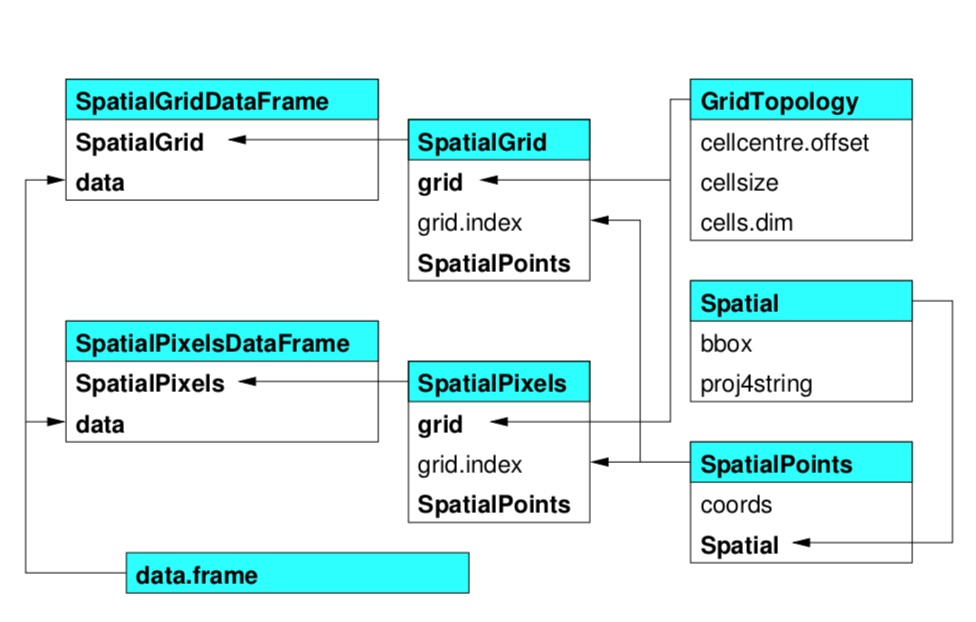
\includegraphics[width=1\textwidth]{figSpatialGrids.png}
\end{center}

\end{frame}

\section{SpatialLines \&
SpatialPolygones}\label{spatiallines-spatialpolygones}

\begin{frame}{Polygons}

\begin{itemize}
\tightlist
\item
  Un objet \emph{Line} = ensemble de coordonnées 2D sans ordre. Un
  \emph{Polygon} = \emph{Line} fermée. \emph{Lines}= liste de
  \emph{Line}.
\item
  Un objet \emph{SpatialLines} = ensemble de listes de coordonnées 2D
  avec ordre. Idem pour \emph{SpatialPolygons}
\item
  \emph{SpatialLinesDataFrame} et \emph{SpatialPolygonsDataFrame} =+
  data.frame dont les lignes associées aux coordonnées.
\end{itemize}

\end{frame}

\begin{frame}[fragile]{Polygons et leur famille}

Les données meuse du package \textbf{sp} contiennent les coordonnées des
bords de la rivière. On les transforme en un objet
\emph{SpatialPolygons} :

\begin{Shaded}
\begin{Highlighting}[]
\KeywordTok{data}\NormalTok{(meuse.riv)}
\KeywordTok{str}\NormalTok{(meuse.riv)}
\NormalTok{##  num [1:176, 1:2] 182004 182137 182252 182314 182332 ...}
\NormalTok{meuse.riv_poly <-}\StringTok{ }\KeywordTok{SpatialPolygons}\NormalTok{(}\KeywordTok{list}\NormalTok{(}\KeywordTok{Polygons}\NormalTok{(}\KeywordTok{list}\NormalTok{(}\KeywordTok{Polygon}\NormalTok{(meuse.riv)), }\DataTypeTok{ID =} \StringTok{"meuse"}\NormalTok{)))}
\KeywordTok{summary}\NormalTok{(meuse.riv_poly )}
\NormalTok{## Object of class SpatialPolygons}
\NormalTok{## Coordinates:}
\NormalTok{##        min      max}
\NormalTok{## x 178304.0 182331.5}
\NormalTok{## y 325698.5 337684.8}
\NormalTok{## Is projected: NA }
\NormalTok{## proj4string : [NA]}
\end{Highlighting}
\end{Shaded}

\end{frame}

\begin{frame}[fragile]{\emph{SpatialPolygons} + \emph{SpatialPoints} +
\emph{SpatialPixels}}

Le tout ensemble:

\begin{Shaded}
\begin{Highlighting}[]

\KeywordTok{layout}\NormalTok{(}\KeywordTok{matrix}\NormalTok{(}\DecValTok{1}\NormalTok{:}\DecValTok{4}\NormalTok{, }\DecValTok{1}\NormalTok{, }\DecValTok{4}\NormalTok{, }\DataTypeTok{byrow =} \OtherTok{TRUE}\NormalTok{))}
\KeywordTok{par}\NormalTok{(}\DataTypeTok{mar =} \KeywordTok{c}\NormalTok{(}\DecValTok{0}\NormalTok{,}\DecValTok{0}\NormalTok{,}\DecValTok{1}\NormalTok{,}\DecValTok{0}\NormalTok{))}
\CommentTok{#plot(meuse_sp, cex = 0.6)}
\KeywordTok{is}\NormalTok{(meuse_sp)}
\NormalTok{## [1] "SpatialPointsDataFrame" "SpatialPoints"         }
\NormalTok{## [3] "Spatial"}

\NormalTok{cc =}\StringTok{ }\KeywordTok{coordinates}\NormalTok{(meuse_sp)}
\NormalTok{meuse.sl =}\StringTok{ }\KeywordTok{SpatialLines}\NormalTok{(}\KeywordTok{list}\NormalTok{(}\KeywordTok{Lines}\NormalTok{(}\KeywordTok{list}\NormalTok{(}\KeywordTok{Line}\NormalTok{(cc)), }\StringTok{"mess"}\NormalTok{)))}
\CommentTok{#plot(meuse.sl)}
\KeywordTok{is}\NormalTok{(meuse.sl)}
\NormalTok{## [1] "SpatialLines" "Spatial"}

\CommentTok{#plot(meuse.riv_poly, col = "grey")}
\KeywordTok{is}\NormalTok{(meuse.riv_poly)}
\NormalTok{## [1] "SpatialPolygons" "Spatial"}

\CommentTok{#image(meuse_spx, col = "grey")}
\KeywordTok{is}\NormalTok{(meuse_spx)}
\NormalTok{## [1] "SpatialPixelsDataFrame" "SpatialPixels"         }
\NormalTok{## [3] "SpatialPointsDataFrame" "SpatialPoints"         }
\NormalTok{## [5] "Spatial"}
\end{Highlighting}
\end{Shaded}

\end{frame}

\begin{frame}{\emph{SpatialPoints} + \emph{SpatialPolygons} +
\emph{SpatialPixels}}

Le tout ensemble:

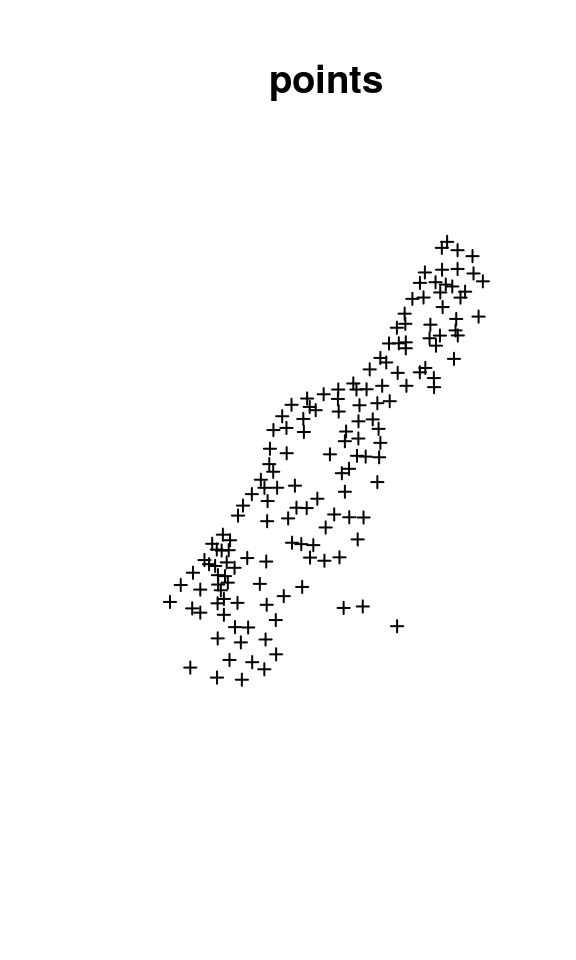
\includegraphics{happyR-230318_files/figure-beamer/faireSpatialPolygonsDataFrame3-1.pdf}
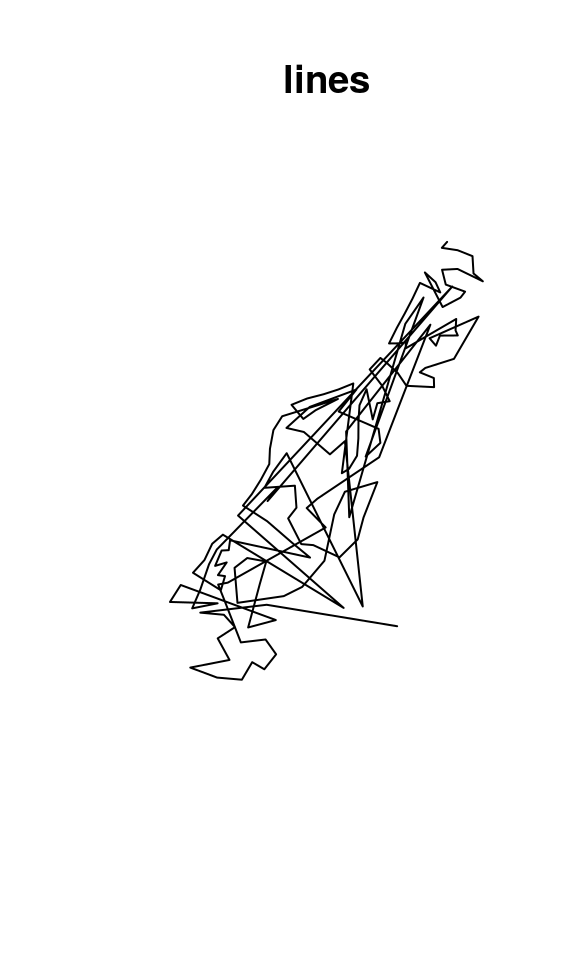
\includegraphics{happyR-230318_files/figure-beamer/faireSpatialPolygonsDataFrame3-2.pdf}
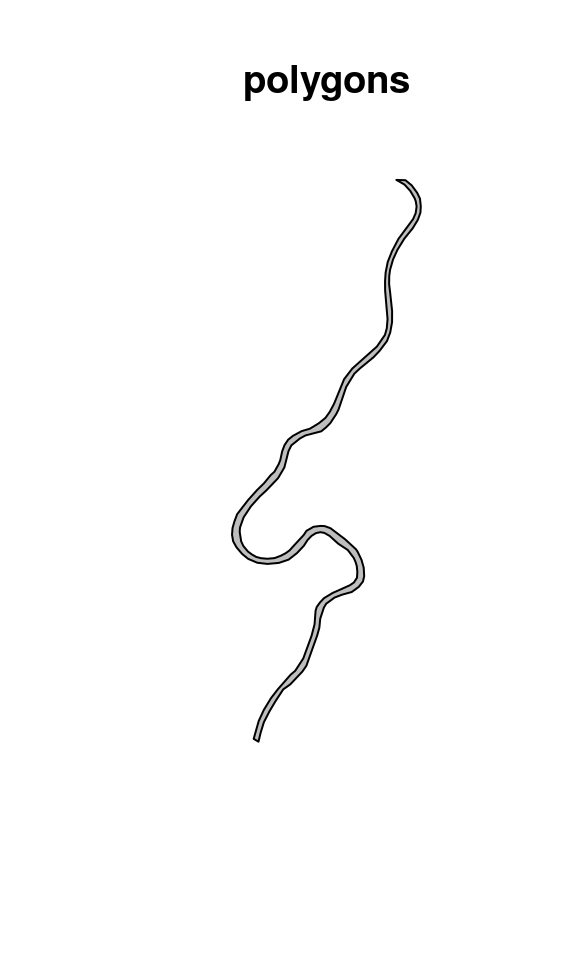
\includegraphics{happyR-230318_files/figure-beamer/faireSpatialPolygonsDataFrame3-3.pdf}
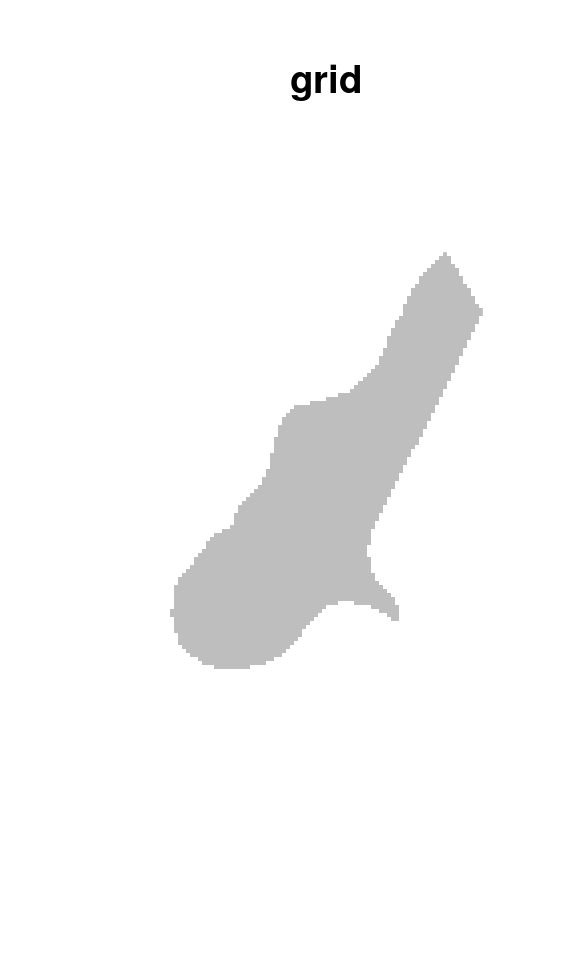
\includegraphics{happyR-230318_files/figure-beamer/faireSpatialPolygonsDataFrame3-4.pdf}

\end{frame}

\begin{frame}{\emph{SpatialPoints} + \emph{SpatialPolygons} +
\emph{SpatialPixels}}

Le tout ensemble:

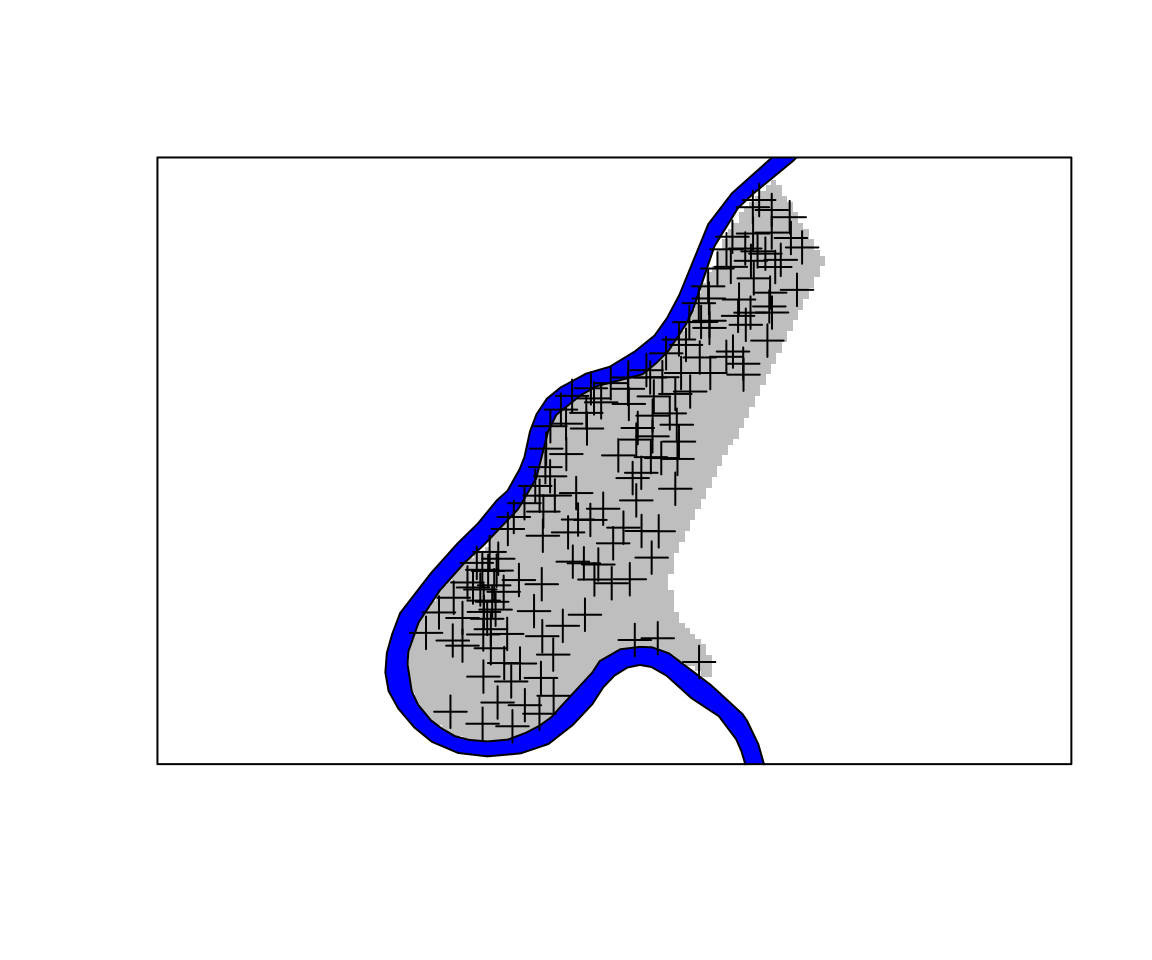
\includegraphics{happyR-230318_files/figure-beamer/faireSpatialPolygonsDataFrame4-1.pdf}

\end{frame}

\begin{frame}[fragile]{Spatial Lines et \emph{ContourLines2SLDF}}

\begin{Shaded}
\begin{Highlighting}[]
\KeywordTok{data}\NormalTok{(volcano)}
\CommentTok{#?ContourLines2SLDF}
\NormalTok{volcano_sl <-}\StringTok{ }\KeywordTok{ContourLines2SLDF}\NormalTok{(}\KeywordTok{contourLines}\NormalTok{(volcano,}\DataTypeTok{nlevels=}\DecValTok{10}\NormalTok{)) }
\KeywordTok{sapply}\NormalTok{(}\KeywordTok{slot}\NormalTok{(volcano_sl, }\StringTok{"lines"}\NormalTok{), function(x) }\KeywordTok{length}\NormalTok{(}\KeywordTok{slot}\NormalTok{(x, }\StringTok{"Lines"}\NormalTok{)))}
\NormalTok{##  [1] 3 4 1 1 1 2 2 3 2 1}
\NormalTok{volcano_sl$level}
\NormalTok{##  [1] 100 110 120 130 140 150 160 170 180 190}
\NormalTok{## Levels: 100 110 120 130 140 150 160 170 180 190}


\NormalTok{col <-}\StringTok{ }\KeywordTok{terrain.colors}\NormalTok{(}\KeywordTok{nlevels}\NormalTok{(volcano_sl$level)) }
\CommentTok{# plot(volcano_sl, bg = "grey70",}
\CommentTok{# col = col[as.numeric(volcano_sl$level)], lwd = 3)}
\end{Highlighting}
\end{Shaded}

\end{frame}

\begin{frame}{Spatial Lines et \emph{ContourLines2SLDF}}

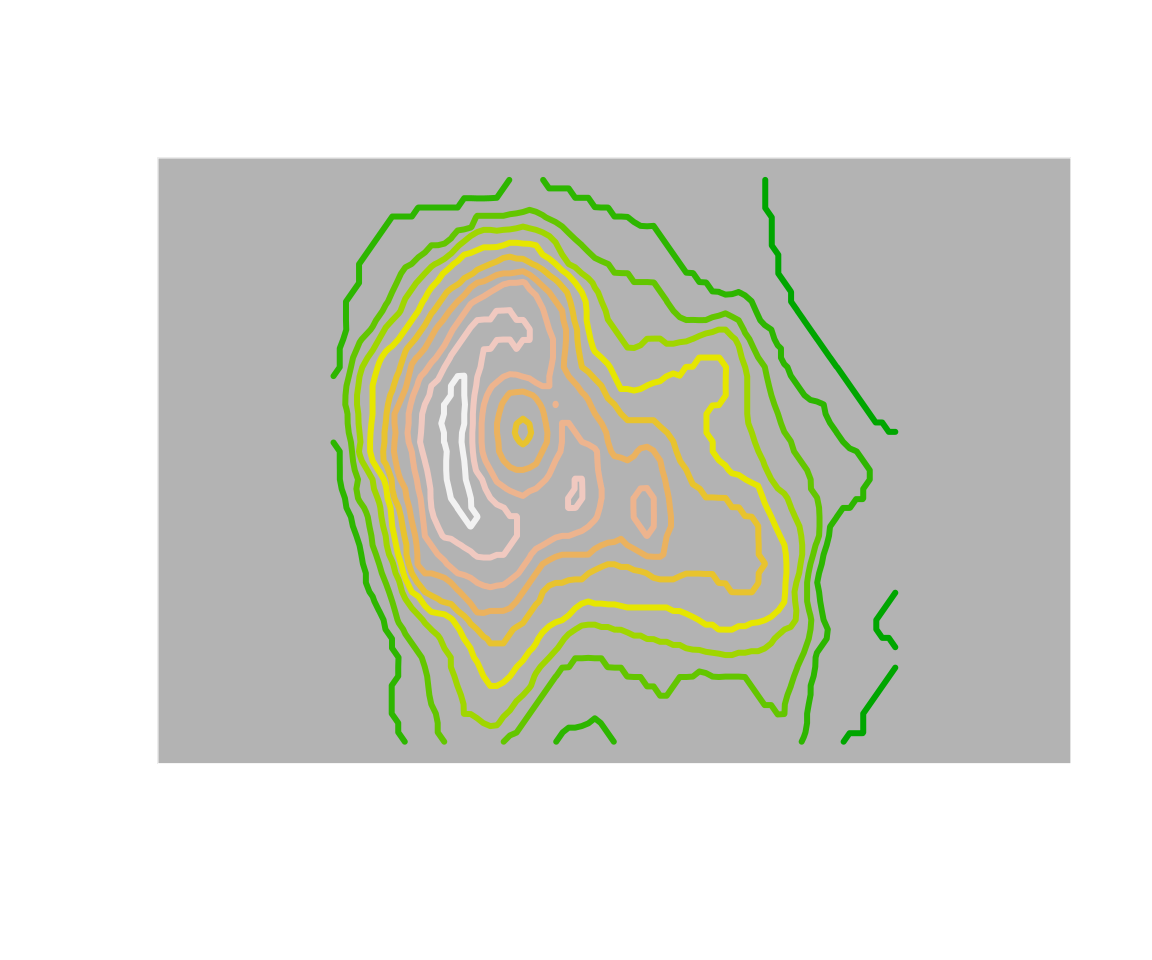
\includegraphics{happyR-230318_files/figure-beamer/faireContourLines2SLDF2-1.pdf}

\end{frame}

\begin{frame}{Exercice 4}

\begin{itemize}
\item
  Quelle est la nature de l'objet \emph{france} obtenu à partir du
  package \emph{Cshapes} dans l'exercice 1 ?
\item
  Créer des lignes de niveaux pour les previsions Chimère de PM25. Les
  transformer en un objet de la famille \emph{SpatialPolygonsDataFrame}.
  Représenter ces lignes de niveaux sur celles obtenues pour
  l'interpolation (``IDW'' ou ``krigeage'') obtenue à partir des
  observations de PM25.
\end{itemize}

\end{frame}

\begin{frame}{Recap ASDAR page 40}

\begin{center}
  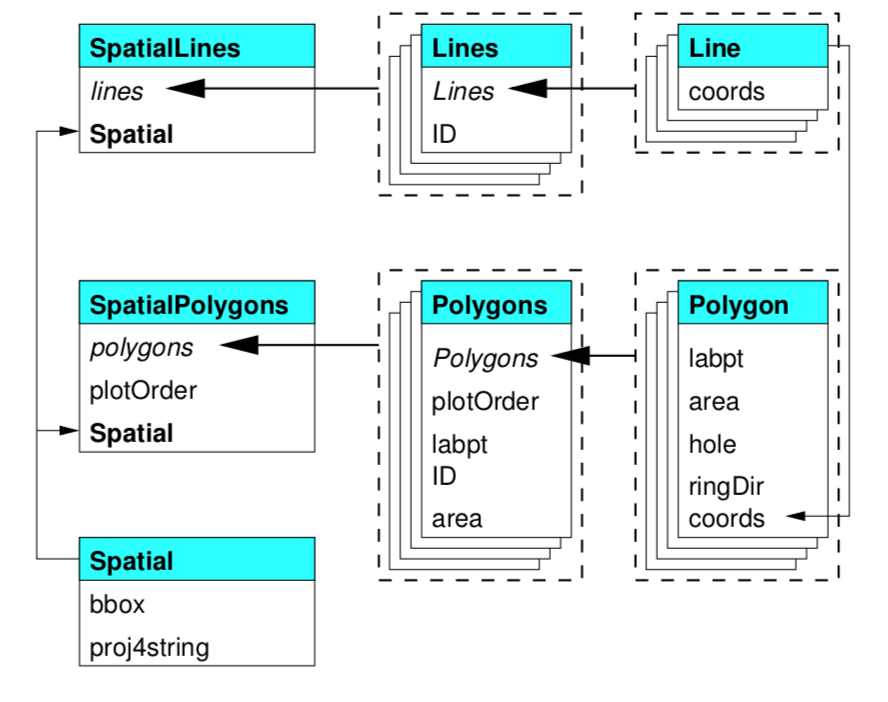
\includegraphics[width=1\textwidth]{figSpatialPolygons.png}
\end{center}

\end{frame}

\end{document}
